\documentclass[a4paper, 10pt, fleqn]{article}

\usepackage{layout}

\title{TKOM - Signale und Systeme}
\author{daniw}
\date{\today}

\begin{document}

\maketitle

\clearpage

\tableofcontents

\clearpage

\section{SW01}
\subsection{Anwendung}
\begin{itemize}
    \item Speicherung von Informationen
    \item Informationsübertragung
    \item Extraktion von Information
    \item Detektion von Ereignissen
\end{itemize}
\subsection{Buch}
Signal- und Systemtheorie - Thomas Frey, Martin Bossert \\
Online verfügbar in HSLU Bibliothek

\section{Einleitung}
\begin{tabular}{|l|l|l|l|}
\hline                         &                   & \multicolumn{2}{|c|}{Amplitude} \\
\hline                         &                   & kontinuierlich    & diskret \\
\hline \multirow{2}{*}{Zeit}   & kontinuierlich    & analog            & \\
\cline{2-4}                    & diskret           &                   & digital   \\
\hline
\end{tabular}

Kontinuierliches System: 
\[ y(t) = H\{x(t)\} \]
Diskretes System: 
\[ y[k] = H\{x[k]\} \qquad k \in \mathbb{N} \]

\subsection{Systeme}
Lineares System: 
\[ H\{a_1 x_1(t) + a_2 x_2(t)\} = a_1 H\{x_1(t)\} + a_2 H\{x_2(t)\}, \qquad a_1, a_2 \in \mathbb{R}(\mathbb{C}) \]
Zeitinvariantes System: 
\[ y(t - t_0) = H\{x(t - t_0)\} \]
LTI-System: linear und zeitinvariant \\\\
Kausales System: 
\[ y(t_0) = H\{x(t \leq t_0)\} \]
Stabilas System:
\[ |x(t)| < \infty \Rightarrow |H\{x(t)\}| < \infty \]

\subsubsection{Beispiele}
Signal $x(t)$ \\
$x(t - \tau$ ist die umf $\tau$ verzögerte Version von $x(t)$. \\\\
\[
    y(t) = \left\{
    \begin{array}{lll}
        x(t) & \text{für} 0 \leq t \leq 1 \\
        0    & \text{für} t < 0, t = 1 \\
    \end{array}
    \right.
\]
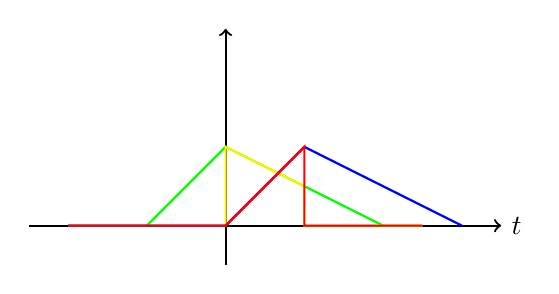
\begin{tikzpicture}
    \draw[thick, ->]        (-2.5,0) -- (3.5,0) node[right] {$t$};
    \draw[thick, ->]        (0,-0.5) -- (0,2.5);
    \draw[thick, green]     (-2,0) -- (-1,0) -- (0,1) -- (2,0) -- (2.5,0);
    \draw[thick, yellow]    (-2,0) -- (0,0) -- (0,1) -- (1,0.5) -- (1,0) -- (2.5,0);
    \draw[thick, blue]      (-2,0) -- (0,0) -- (1,1) -- (3,0);
    \draw[thick, red]       (-2,0) -- (0,0) -- (1,1) -- (1,0) -- (2.5,0);
\end{tikzpicture}\\
$\to$ nicht zeitinvariant $\to$ kein LTI-System

\section{Signale}
Zeitliche Verschiebung
\[ x(t - t_0) \]
Zeitliche Spiegelung
\[ x(-t) \]
Zeitliche Skalierung
\[ x(a \cdot t) \]
Komplexe Signale
\[ x(t) = x_R(t) + j \cdot x_I(t) = Re(x(t)) + j \cdot Im(x(t)) = |x(t)| \cdot e^{j \angle x(t)} \]
Gerade Signale
\[ x(t) = x(-t) \]
Ungerade Signale
\[ x(t) = -x(-t) \]
Zerlegung in geraden und ungeraden Anteil
\[ x_g(t) = \frac{1}{2} \cdot \left(x(t) - x(-t)\right) \]
\[ x_u(t) = \frac{1}{2} \cdot \left(x(t) + x(-t)\right) \]
\[ x(t) = x_g(t) + x_u(t) \]
Konjugiert gerade Signale
\[ x(t) = x^{\star}(-t) \]
Konjugiert ungerade Signale
\[ x(t) = -x^{\star}(-t) \]
Periodische Signale
\[ x(t) = x(t + n \cdot T_p) \qquad n \in \mathbb{Z} \]
Zeitbegrenzte Signale
\[ x(t) = 0 \qquad \text{für $t < t_1$ oder $t > t_2$} \]

\subsection{Spezielle Signale}
Zeitdiskreter Dirac-Impuls
\[
\sigma[k] = \left\{
    \begin{array}{ll}
        1, & k = 0 \\
        0, & k \neq 0
    \end{array}
\right.
\]
Zeitdiskrete Sprungfunktion
\[
\varepsilon[k] = \left\{
    \begin{array}{ll}
        1, & k \geq 0 \\
        0, & k < 0
    \end{array}
\right.
\]
Kontinuierliche Sprungfunktion
\[
\varepsilon(t) = \left\{
    \begin{array}{ll}
        1, & t > 0 \\
        0, & t < 0
    \end{array}
\right.
\]
Zeitdiskrete Signumfolge
\[
\sgn[k] = \left\{
    \begin{array}{ll}
        1,  & k > 0 \\
        0,  & k = 0 \\
        -1, & k < 0
    \end{array}
\right.
\]
Kontinuierlicher Rechteckimpuls
\[
\rect_T(t) = \left\{
    \begin{array}{ll}
        1, & |t| < \frac{T}{2} \\
        0, & |t| > \frac{T}{2}
    \end{array}
\right.
\]
Reelle Exponentialfunktion
\[ x(t) = A \cdot e^{\alpha t} \qquad \alpha < 0 \to \text{ abklingend} \qquad \alpha > 0 \to \text{ aufklingend} \]
Komplexe Exponentialfunktion
\[ x(t) = A \cdot e^{\alpha t} \cdot e^{j \omega_0 t} = \underbrace{|A| \cdot e^{\sigma t}}_{\text{Einhüllende}} \cdot \underbrace{e^{j(\omega_0 t + \varphi_0)}}_{\text{komplexe Schwingung}} \]
si-Funktion
\[ \si(t) = \frac{\sin(t)}{t} \]

\end{document}
